\subsection{StyleCLIP}
\begin{frame}[allowframebreaks]{StyleCLIP}
    \textbf{StyleCLIP} combines CLIP (Contrastive Language-Image Pretraining) with StyleGAN to generate images based on text prompts, allowing for fine-grained control over image attributes.

    \begin{itemize}
        \item \textbf{CLIP Embeddings:} Uses CLIP to encode text prompts into embeddings that capture semantic information.
        \item \textbf{StyleGAN Manipulation:} Applies these embeddings to manipulate the latent space of StyleGAN, enabling the generation of images that match the desired attributes described in the text.
        \item \textbf{Applications:} Useful for tasks like image editing, attribute manipulation, and creative content generation.
        \item \textbf{Benefits:} Generates diverse images from textual descriptions without retraining StyleGAN.
        \item \textbf{Costs:} Bound to the attributes StyleGAN already models; edits outside its latent space either fail or introduce artifacts.
    \end{itemize}
\framebreak
    \begin{figure}
        \centering
        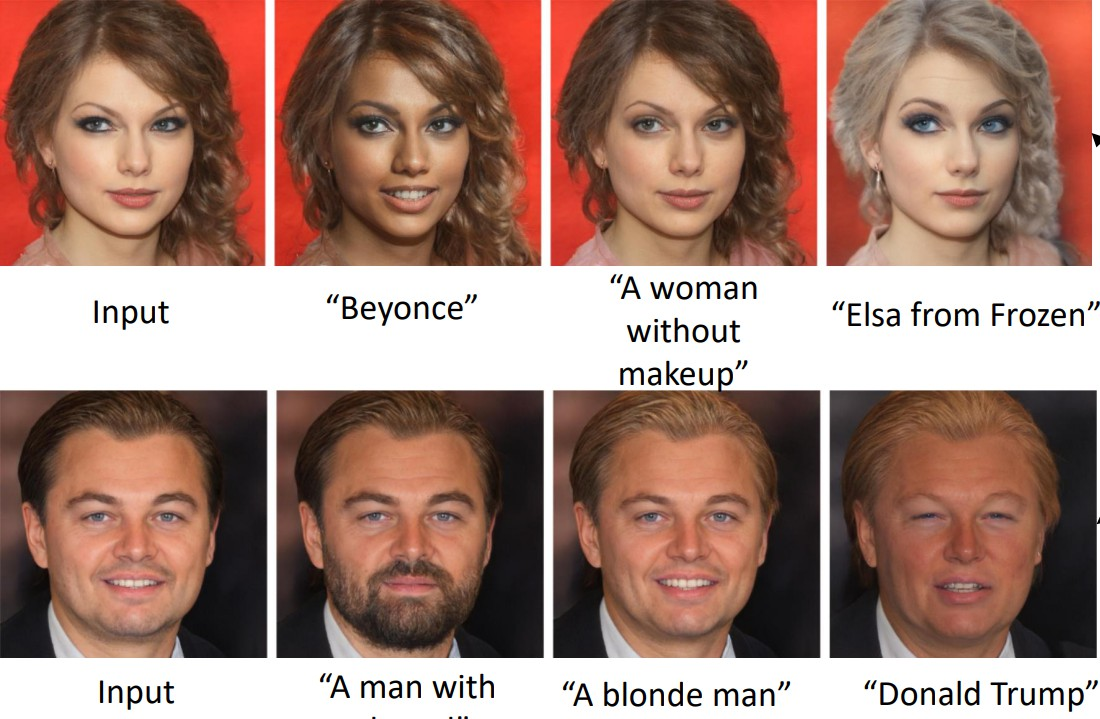
\includegraphics[width=1\textwidth,height=0.85\textheight,keepaspectratio]{images/video/slide_65_1_img.jpg}
    \end{figure}
    {\footnotesize{[StyleCLIP: Text-Driven Manipulation of StyleGAN Imagery, Patashnik et al., ICCV 2021]}}
\framebreak
    \begin{figure}
        \centering
        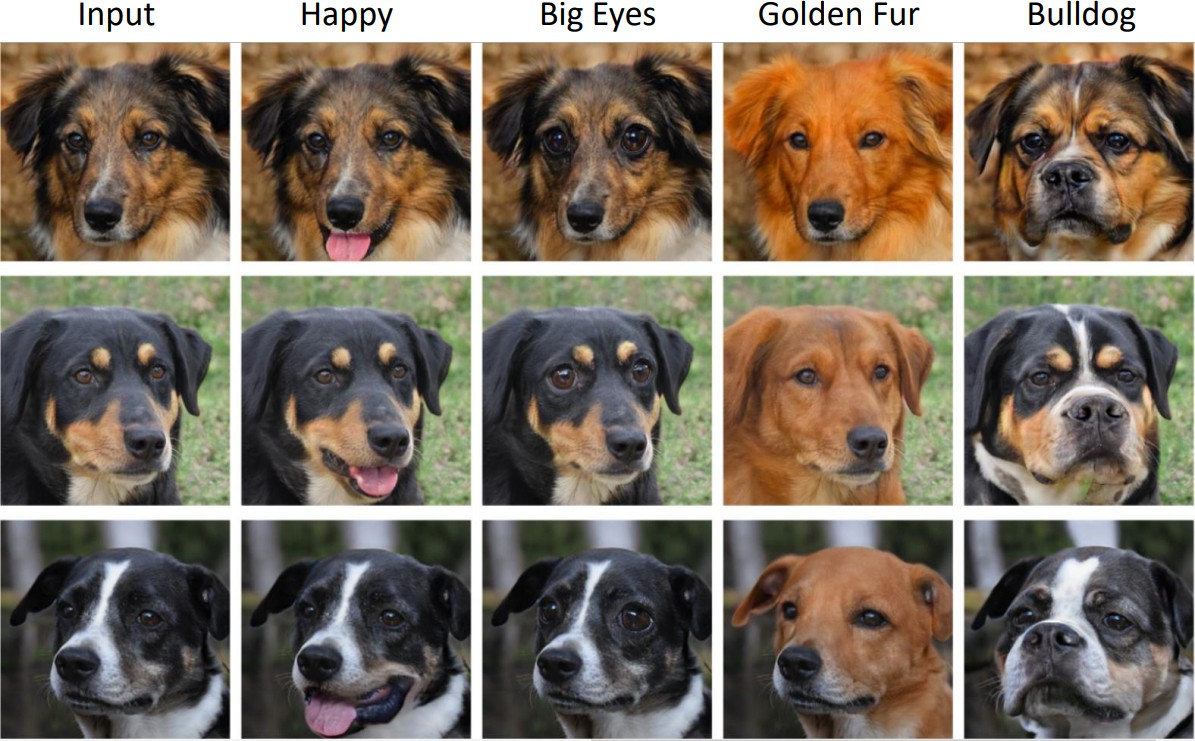
\includegraphics[width=1\textwidth,height=0.85\textheight,keepaspectratio]{images/video/slide_66_1_img.jpg}
    \end{figure}
    {\footnotesize{[StyleCLIP, Patashnik et al., ICCV 2021, Fig.~8 (AFHQ dogs)]}}

\framebreak
    \begin{figure}
        \centering
        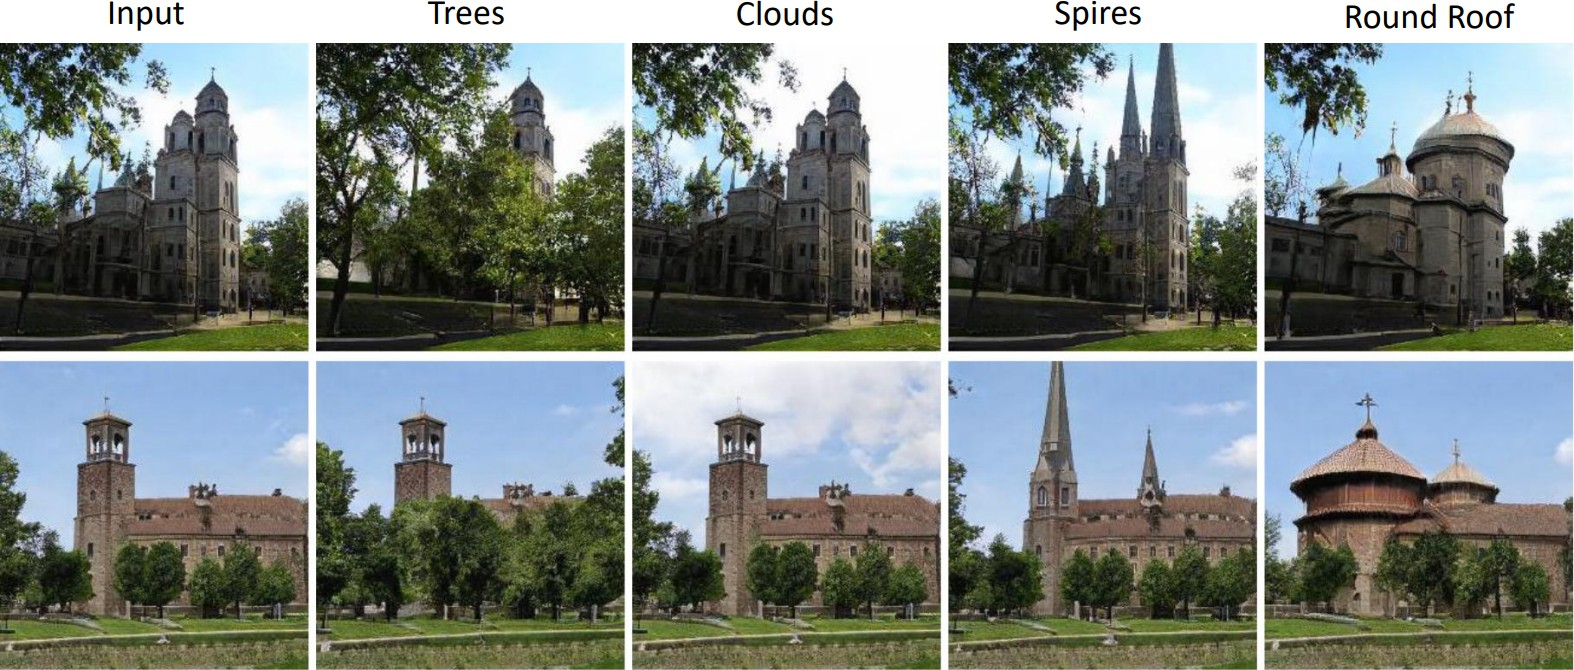
\includegraphics[width=1\textwidth,height=0.85\textheight,keepaspectratio]{images/video/slide_67_1_img.jpg}
    \end{figure}
    {\footnotesize{[StyleCLIP, Patashnik et al., ICCV 2021, Fig.~19 (LSUN Church)]}}
\end{frame}